\documentclass[t, aspectratio=169]{beamer}
\usepackage{amsmath,amsfonts,amsthm,amstext,amssymb, xcolor, tikz, pgf, mathrsfs, polynom, pifont, tabto}

% ----------------------------------------------------------
% Theme Setup

% Use Metropolis Theme
\usetheme[numbering=fraction]{metropolis}
\setbeamertemplate{blocks}[rounded][shadow=false]
\makeatletter
\setlength{\metropolis@titleseparator@linewidth}{1pt}
\makeatother

% Define Colors
\definecolor{chargerblue}{HTML}{002764}
\definecolor{chargerred}{HTML}{e02034}
\definecolor{bggray}{HTML}{d0d3d4}

% Set Colors
\setbeamercolor{title}{fg=chargerblue}
\setbeamercolor{background canvas}{bg=white}
\setbeamercolor{title separator}{fg=chargerred}
\setbeamercolor{structure}{fg=chargerblue}
\setbeamercolor{frametitle}{fg=white, bg=chargerblue}
\setbeamercolor*{normal text}{fg=chargerblue}
\setbeamercolor*{block body}{bg=bggray}
\setbeamercolor*{block title}{bg=chargerblue, fg=white}
% ----------------------------------------------------------

% ----------------------------------------------------------
% Custom Definitions, Commands, Environments, etc.

% Sets of numbers
\def\R{\mathbb{R}} % The reals
\def\N{\mathbb{N}} % The naturals
\def\Z{\mathbb{Z}} % The integers
\def\Q{\mathbb{Q}} % The rationals

% Blank space
\newcommand{\blank}[1]{\underline{\hspace{#1}}} % Blank space

% Change font colors
\newcommand{\cyan}[1]{{\color{cyan}{#1}}} % Changes font to cyan
\newcommand{\red}[1]{{\color{red}{#1}}} % Changes font to red
\newcommand{\magenta}[1]{{\color{magenta}{#1}}} % Changes font to magenta
\newcommand{\orange}[1]{{\color{orange}{#1}}} % Changes font to orange
\newcommand{\yellow}[1]{{\color{yellow}{#1}}} % Changes font to yellow
\newcommand{\violet}[1]{{\color{violet}{#1}}} % Changes font to violet
\newcommand{\green}[1]{{\color{green}{#1}}} % Changes font to green
\newcommand{\blue}[1]{{\color{blue}{#1}}} % Changes font to blue
\newcommand{\white}[1]{{\color{white}{#1}}} % Changes font to white

% Fitted inclusion symbols
\newcommand{\fp}[1]{\left({#1}\right)} % Fitted parentheses around content
\newcommand{\fb}[1]{\left[{#1}\right]} % Fitted brackets
\newcommand{\lhoi}[1]{\left({#1}\right]} % Left half-open interval
\newcommand{\rhoi}[1]{\left[{#1}\right)} % Right half-open interval
\newcommand{\set}[1]{\left\{{#1}\right\}} % Fitted braces (useful for sets)
\newcommand{\av}[1]{\left|{#1}\right|} % Fitted absolute value bars

% Augmented Matrix Environment
\newenvironment{amatrix}[1]{%
	\left[\begin{array}{@{}*{#1}{c}|c@{}}
	}{%
	\end{array}\right]
}

% Miscellaneous
\def\then{\Rightarrow}
\def\to{\rightarrow}
\def\d{^{\circ}}
\newcommand{\?}{\stackrel{?}{=}}
\newcommand{\cmark}{\text{ \ding{51}}}
\newcommand{\xmark}{\text{ \ding{55}}}

% Coordinate Plane (Four-Quadrant)
\def\coordplane {
	\begin{tikzpicture}        \draw[step=0.25cm,black,very thin,opacity=0.25] (-2.5cm, -2.5cm) grid (2.5cm, 2.5cm);
		\draw[<->,thick,black] (-2.5cm, 0) -- (2.5cm, 0) node[anchor=north west,pos=0.94,font=\scriptsize]{$x$};
		\draw[<->,thick,black] (0,-2.5cm) -- (0, 2.5cm) node[anchor=south east,font=\scriptsize,pos=0.94]{$y$};
	\end{tikzpicture}
}

% Coordinate Plane (One-Quadrant)
\def\onequad {
	\begin{tikzpicture}
		\draw[step=0.25cm, black, very thin, opacity=0.25] (0,0) grid (7.5cm,5cm);
		\draw[->, thick, black] (0,0) -- (7.5cm, 0) node[anchor=north west,font=\scriptsize,pos=0.94]{$x$};
		\draw[->, black, thick] (0,0) -- (0,5cm) node[anchor=south east,font=\scriptsize,pos=0.94]{$y$};
	\end{tikzpicture}
}
% ----------------------------------------------------------

% ----------------------------------------------------------
% Presentation Information
\title[3-3]{Measures of Position}
\subtitle{Section 3-3}
\author{Jacob Ayers}
\institute{Lesson \#7}
\date{MAT 110}
% ----------------------------------------------------------

\begin{document}
	
	% Slide 1 (Title Slide)
	\begin{frame}
		\titlepage
	\end{frame}
	
	% Slide 2 (Objectives)
	\begin{frame}{Objectives}
		\begin{itemize}
			\item Find the $z$ score for a value in a data set
			\item Find the percentile rank for a value in a data set
			\item Find data values corresponding to given percentile ranks
			\item Find $Q_1$ and $Q_3$ for a data set
			\item Identify outliers in data sets
		\end{itemize}
	\end{frame}

	\begin{frame}{Measures of Position}
		Measures of position locate the relative position of a data value. \pause
		
		We will be looking at two measures of position in this lesson: \begin{itemize}
			\item Standard ($z$) score
			\item Percentile rank
		\end{itemize}
	\end{frame}

	\begin{frame}{Standard Score}
		The standard score allows us to compare relative positions of unrelated data values. \pause
		
		For example, say we want to compare a student's performance on a math test and an English test. \pause
		
		The standard score (also known as the $z$ score) tells how many standard deviations a data value is above or below the mean. \pause
		
		Formulas: \\
		$z = \dfrac{X - \overline{X}}{s}$ for samples \\
		$z = \dfrac{X - \mu}{\sigma}$ for populations
	\end{frame}

	\begin{frame}{Standard Score}
		A student scored 85 on an English test while the mean score of all the students was 76 and the standard deviation was $4$. She also scored 42 on a French test where the class mean was 36 and the standard deviation was $3$. Compare the relative positions on the two tests.
		
		\onslide<2->{First, find the $z$-scores:} \vspace{-18pt}
		\begin{columns}
			\begin{column}{0.5\textwidth}
				\begin{flalign*}
					\onslide<3->{z &= \dfrac{X - \overline{X}}{s}} & \\
					\onslide<4->{&= \dfrac{85 - 76}{4}} & \\
					\onslide<5->{&= 2.25}
				\end{flalign*}
			\end{column}
			\begin{column}{0.5\textwidth}
				\begin{flalign*}
					\onslide<3->{z &= \dfrac{X - \overline{X}}{s}} & \\
					\onslide<4->{&= \dfrac{42 - 36}{3}} & \\
					\onslide<5->{&= 2.00}
				\end{flalign*}
			\end{column}
		\end{columns}
		\onslide<6->{Based on the results, our student had a higher relative position on the English test.}
	\end{frame}

	\begin{frame}{Standard Score}
		If the average number of vacation days for a selection of various countries has a mean of 29.4 days and a standard deviation of 8.6 days, find the $z$ score for the United States, which has an average number of $13$ days per year.
		\begin{flalign*}
			\onslide<2->{z &= \dfrac{X - \overline{X}}{s}} & \\
			\onslide<3->{&= \dfrac{13 - 29.4}{8.6}} & \\
			\onslide<4->{&= \dfrac{-16.4}{8.6}} & \\
			\onslide<5->{&= -1.91}
		\end{flalign*}
	\end{frame}

	\begin{frame}{Standard Score}
		The average teacher's salary in a particular state is \$54,166. If the standard deviation \$10,200, find the salary associated with a $z$ score of $-1.6$. \begin{flalign*}
			\onslide<2->{z &= \dfrac{X - \mu}{\sigma}} & \\
			\onslide<3->{-1.6 &= \dfrac{X - 54166}{10200}} & \\
			\onslide<4->{-16320 &= X - 54166} & \\
			\onslide<5->{X &= 37846}
		\end{flalign*}
	\onslide<6->{So a $z$ score of $-1.6$ corresponds to a salary of \$37,846.}
	\end{frame}

	\begin{frame}{Percentile Rank}
		Percentile ranks divide a data set into 100 equal groups. \pause
		
		For example, say you score in the 80th percentile on a physical fitness test. \pause
		
		This means that 80\% of those who took the test scored lower than you, and 20\% scored higher than you. \pause
		
		Notation: $P_1, P_2, \dots, P_{99}$ 
	\end{frame}

	\begin{frame}{Percentile Rank}
		Often, graphs and tables showing percentiles for various measures have already been created, and we use them to check the percentile rank of a given measurement. \pause
		
		Examples: standardized test score, height/weight of children at a given age, etc. (see pp. 150-151) \pause
		
		Important Note: A \textit{percentile} and a \textit{percentage} are not the same thing! \pause
		
		Example: Say you get a score of 72/100 on a math test. This means your \textit{percentage} score was 72\%. This does \textit{not} mean that you scored in the 72nd percentile. Perhaps the median score was 85; in this case, you actually scored below the 50th \textit{percentile}.
	\end{frame}

	\begin{frame}{Percentile Ranks}
		To calculate the percentile rank for a given value $X$ in a data set, use the formula $$\text{Percentile} = \dfrac{\text{(number of values below $X$)} + 0.5}{\text{total number of values}} \cdot 100$$ \pause
		
		Note: This means we must order the data values from lowest to highest before calculating the percentile. \pause
		
		Note: We round up to the nearest whole number when calculating percentages. Example: $28.21$ is considered the 29th percentile.
	\end{frame}

	\begin{frame}{Percentile Ranks}
		The data show the population (in thousands) for a recent year of a sample of cities in South Carolina.
		
		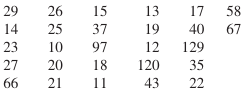
\includegraphics[width=2in]{carolina-data.png}
		
		Find the percentile rank for 58. \pause
		
		First, sort from lowest to highest: \\
		$10, 11, 12, 13, 14, 15, 17, 18, 19, 20, 21, 22, 23, 25, 26, 27, 29, 35, 37, 40, 43, 58, 66, 67, 97,$ \\ $120, 129$ \pause
	
		There are $21$ values less than $58$, so the percentile rank is $\dfrac{21.5}{27} \cdot 100 = 79.62$. We round this up, and say that $58$ is in the 80th percentile.
	\end{frame}

	\begin{frame}{Percentile Rank}
		Refer to the previous data set. Find the percentile rank of $21$. \pause
		
		$10, 11, 12, 13, 14, 15, 17, 18, 19, 20, 21, 22, 23, 25, 26, 27, 29, 35, 37, 40, 43, 58, 66, 67, 97,$ \\ $120, 129$ \pause
		
		There are $10$ values less than $21$, so the percentile rank is $\dfrac{10.5}{27} \cdot 100 = 38.89$. We round this up, and say that $21$ is in the 39th percentile. \pause
	\end{frame}

	\begin{frame}{Percentile Rank}
		Now that we know how to calculate percentile ranks, we move to finding data values corresponding to a given percentile rank.
		
		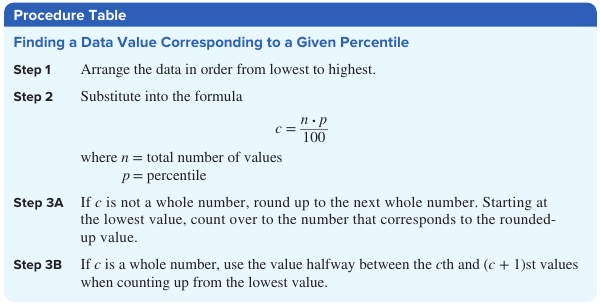
\includegraphics[width=4in]{perc-proc.png}
	\end{frame}

	\begin{frame}{Percentile Rank}
		Refer to the data set below. Find the value corresponding to the 75th percentile and the 90th percentile.
		
		\onslide<2->{$10, 11, 12, 13, 14, 15, 17, 18, 19, 20, 21, 22, 23, 25, 26, 27, 29, 35, 37, 40, 43, 58, 66, 67, 97,$ \\ $120, 129$} \vspace{12pt}
		
		\begin{columns}
			\begin{column}{0.5\textwidth}
				\onslide<3->{$c = \dfrac{27 \times 75}{100}$} \\
				\onslide<4->{$c = 20.25 \uparrow 21$} \\
				\onslide<5->{The 21st value is 43, so the 75th percentile corresponds to 43.}
			\end{column}
			\begin{column}{0.5\textwidth}
				\onslide<3->{$c = \dfrac{27 \times 90}{100}$} \\
				\onslide<4->{$c = 24.3 \uparrow 25$} \\
				\onslide<5->{The 25th value is 97, so the 90th percentile corresponds to 97.}
			\end{column}
		\end{columns}
	\end{frame}

	\begin{frame}{Percentile Rank - $Q_1$ and $Q_3$}
		The 25th percentile is known as the \textit{first quartile}, and is denoted by $Q_1$. \pause
		
		The 75th percentile is known as the \textit{third quartile}, and is denoted by $Q_3$. \pause
		
		Note: Graphing calculators will find these values for you (see last week's videos). \pause
		
		To find $Q_1$ and $Q_3$ by hand: \begin{enumerate}[1)]
			\item Arrange data from lowest to highest, and find the median as we did before.
			\item Find the median of values below the median; this is $Q_1$
			\item Find the median of values above the median; this is $Q_3$
		\end{enumerate} \pause
	
		The \textit{interquartile range} is the difference between the third and first quartiles. \\
		$IQR = Q_3 - Q_1$
	\end{frame}

	\begin{frame}{Percentile Rank - $Q_1$ and $Q_3$}
		Find $Q_1$, $Q_3$, and the interquartile range for the data below.
		
		\onslide<2->{$10, 11, 12, 13, 14, 15, 17, 18, 19, 20, 21, 22, 23, 25, 26, 27, 29, 35, 37, 40, 43, 58, 66, 67, 97,$ \\ $120, 129$} \vspace{12pt}
		
		\onslide<3->{First, find the median (25)}
		
		\onslide<4->{$Q_1$ is the median of all data values below 25 (17)}
		
		\onslide<5->{$Q_3$ is the median of all data values above 25 (43)}
		
		\onslide<6->{$IQR = 43 - 17 = 26$}
	\end{frame}

	\begin{frame}{Outliers}
		An \textit{outlier} is an extremely high or an extremely low value when compared with the rest of the data.
		
		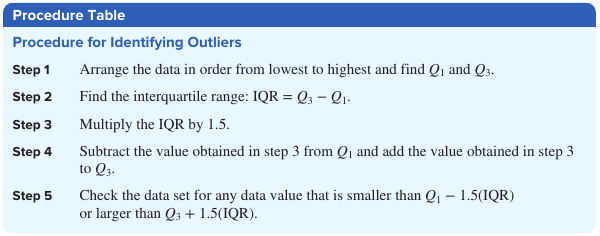
\includegraphics[width=4.5in]{outlier-proc.png}
	\end{frame}

	\begin{frame}{Outliers}
		Check the following data set for outliers.
		
		$5, 6, 12, 13, 15, 18, 22, 50$ \pause
		
		First, find the median (14), $Q_1$ (9), and $Q_3$ (20) \pause
		
		So the interquartile range is $20 - 9 = 11$; $1.5 \times 11 = 16.5$ \pause
		
		Lower boundary: $9 - 16.5 = -7.5$; Upper boundary: $20 + 16.5 = 36.5$ \pause
		
		50 is larger than the upper boundary, so it is an outlier.
	\end{frame}

	\begin{frame}{Outliers}
		Check the following data for outliers.
		
		$19, 21, 25, 28, 29, 32, 34, 46$ \pause
		
		First, find the median (28.5), $Q_1$ (23), and $Q_3$ (33) \pause
		
		So the IQR is $33 - 23 = 10$; $1.5 \times 10 = 15$ \pause
		
		Lower boundary: $23 - 15 = 8$; Upper boundary: $33 + 15 = 48$ \pause
		
		There are no outliers.
	\end{frame}

	\begin{frame}{Next Steps}
		\begin{itemize}
			\item Read 3-4
			\item Watch Video Lesson \#8
			\item Begin preparing for Midterm 1 (Study Guide is available on Moodle)
		\end{itemize}
	
		\vfill
		
		Thanks for watching!
	\end{frame}
	
\end{document}